\documentclass[border=5pt]{standalone}
\usepackage[utf8]{inputenc}
\usepackage{amssymb}
\usepackage{amsmath}
\usepackage{tikz}
\usetikzlibrary{arrows.meta}

\begin{document}
\nopagecolor
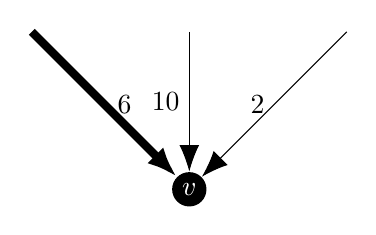
\begin{tikzpicture}
    \node[circle, inner sep=2pt, fill] (v) at (0, 0) {\color{white} $v$};
    \draw [-{Latex[scale=2]}] (0, 2) -- node[left]{10} (v);
    \draw [-{Latex[scale=2]}] (2, 2) -- node[left]{2} (v);
    \draw [-{Latex[scale=0.66]}, line width=3pt] (-2, 2) -- node[right]{6} (v);
\end{tikzpicture}
\hspace{0.25in}
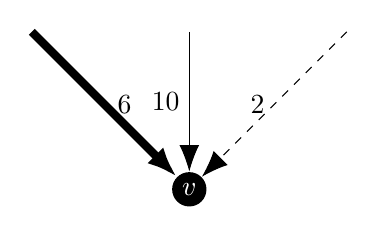
\begin{tikzpicture}
    \node[circle, inner sep=2pt, fill] (v) at (0, 0) {\color{white} $v$};
    \draw [-{Latex[scale=2]}] (0, 2) -- node[left]{10} (v);
    \draw [-{Latex[scale=2]}, dashed] (2, 2) -- node[left]{2} (v);
    \draw [-{Latex[scale=0.66]}, line width=3pt] (-2, 2) -- node[right]{6} (v);
\end{tikzpicture}
\end{document}